\section{Resultados: respuestas a P1--P8}\label{sec:resultados}

Cada pregunta se responde con una frase, las cifras con su IC y $n$, la figura
que la ilustra, la distinción entre lo que es un resultado del modelo y lo que
depende de supuestos, y sus limitaciones. Las figuras muestran medias entre
réplicas con barras de IC del 95~\%; los números de las figuras usan punto
decimal.

% ---------------------------------------------------------------------------
\subsection{P1 · Operativa actual y cuello de botella}

\textbf{Respuesta.} Con la operativa actual (X0: 3 tornos por puerta, FIFO,
perfil base y conflictos, relecturas y averías activas) las esperas en los
tornos son cortas y nadie espera 10~minutos, pero los tornos trabajan cerca de
su límite en la media hora punta y son el cuello de botella de la entrada.

\begin{table}[htbp]
\centering\small
\caption{Operativa actual (X0, $n=180$).}
\label{tab:p1}
\begin{tabular}{@{}lr@{}}
\toprule
Indicador & Valor \\
\midrule
Espera media en cola & 0,192 $\pm$ 0,008~min (unos 11,5~s) \\
Percentil 95 de la espera & 1,150 $\pm$ 0,068~min \\
Público que espera menos de 10~min & 100,0~\% en las 180 réplicas \\
Máximo de personas en la cola de una puerta & 135 $\pm$ 6 \\
Utilización de los tornos & 40,43 $\pm$ 0,01~\% \\
Tiempo de acceso (llegada a la cola $\to$ asiento) & 1,972 $\pm$ 0,008~min \\
Entrada tardía & 4,578 $\pm$ 0,052~\% \\
\bottomrule
\end{tabular}
\end{table}

\begin{figure}[htbp]
\centering
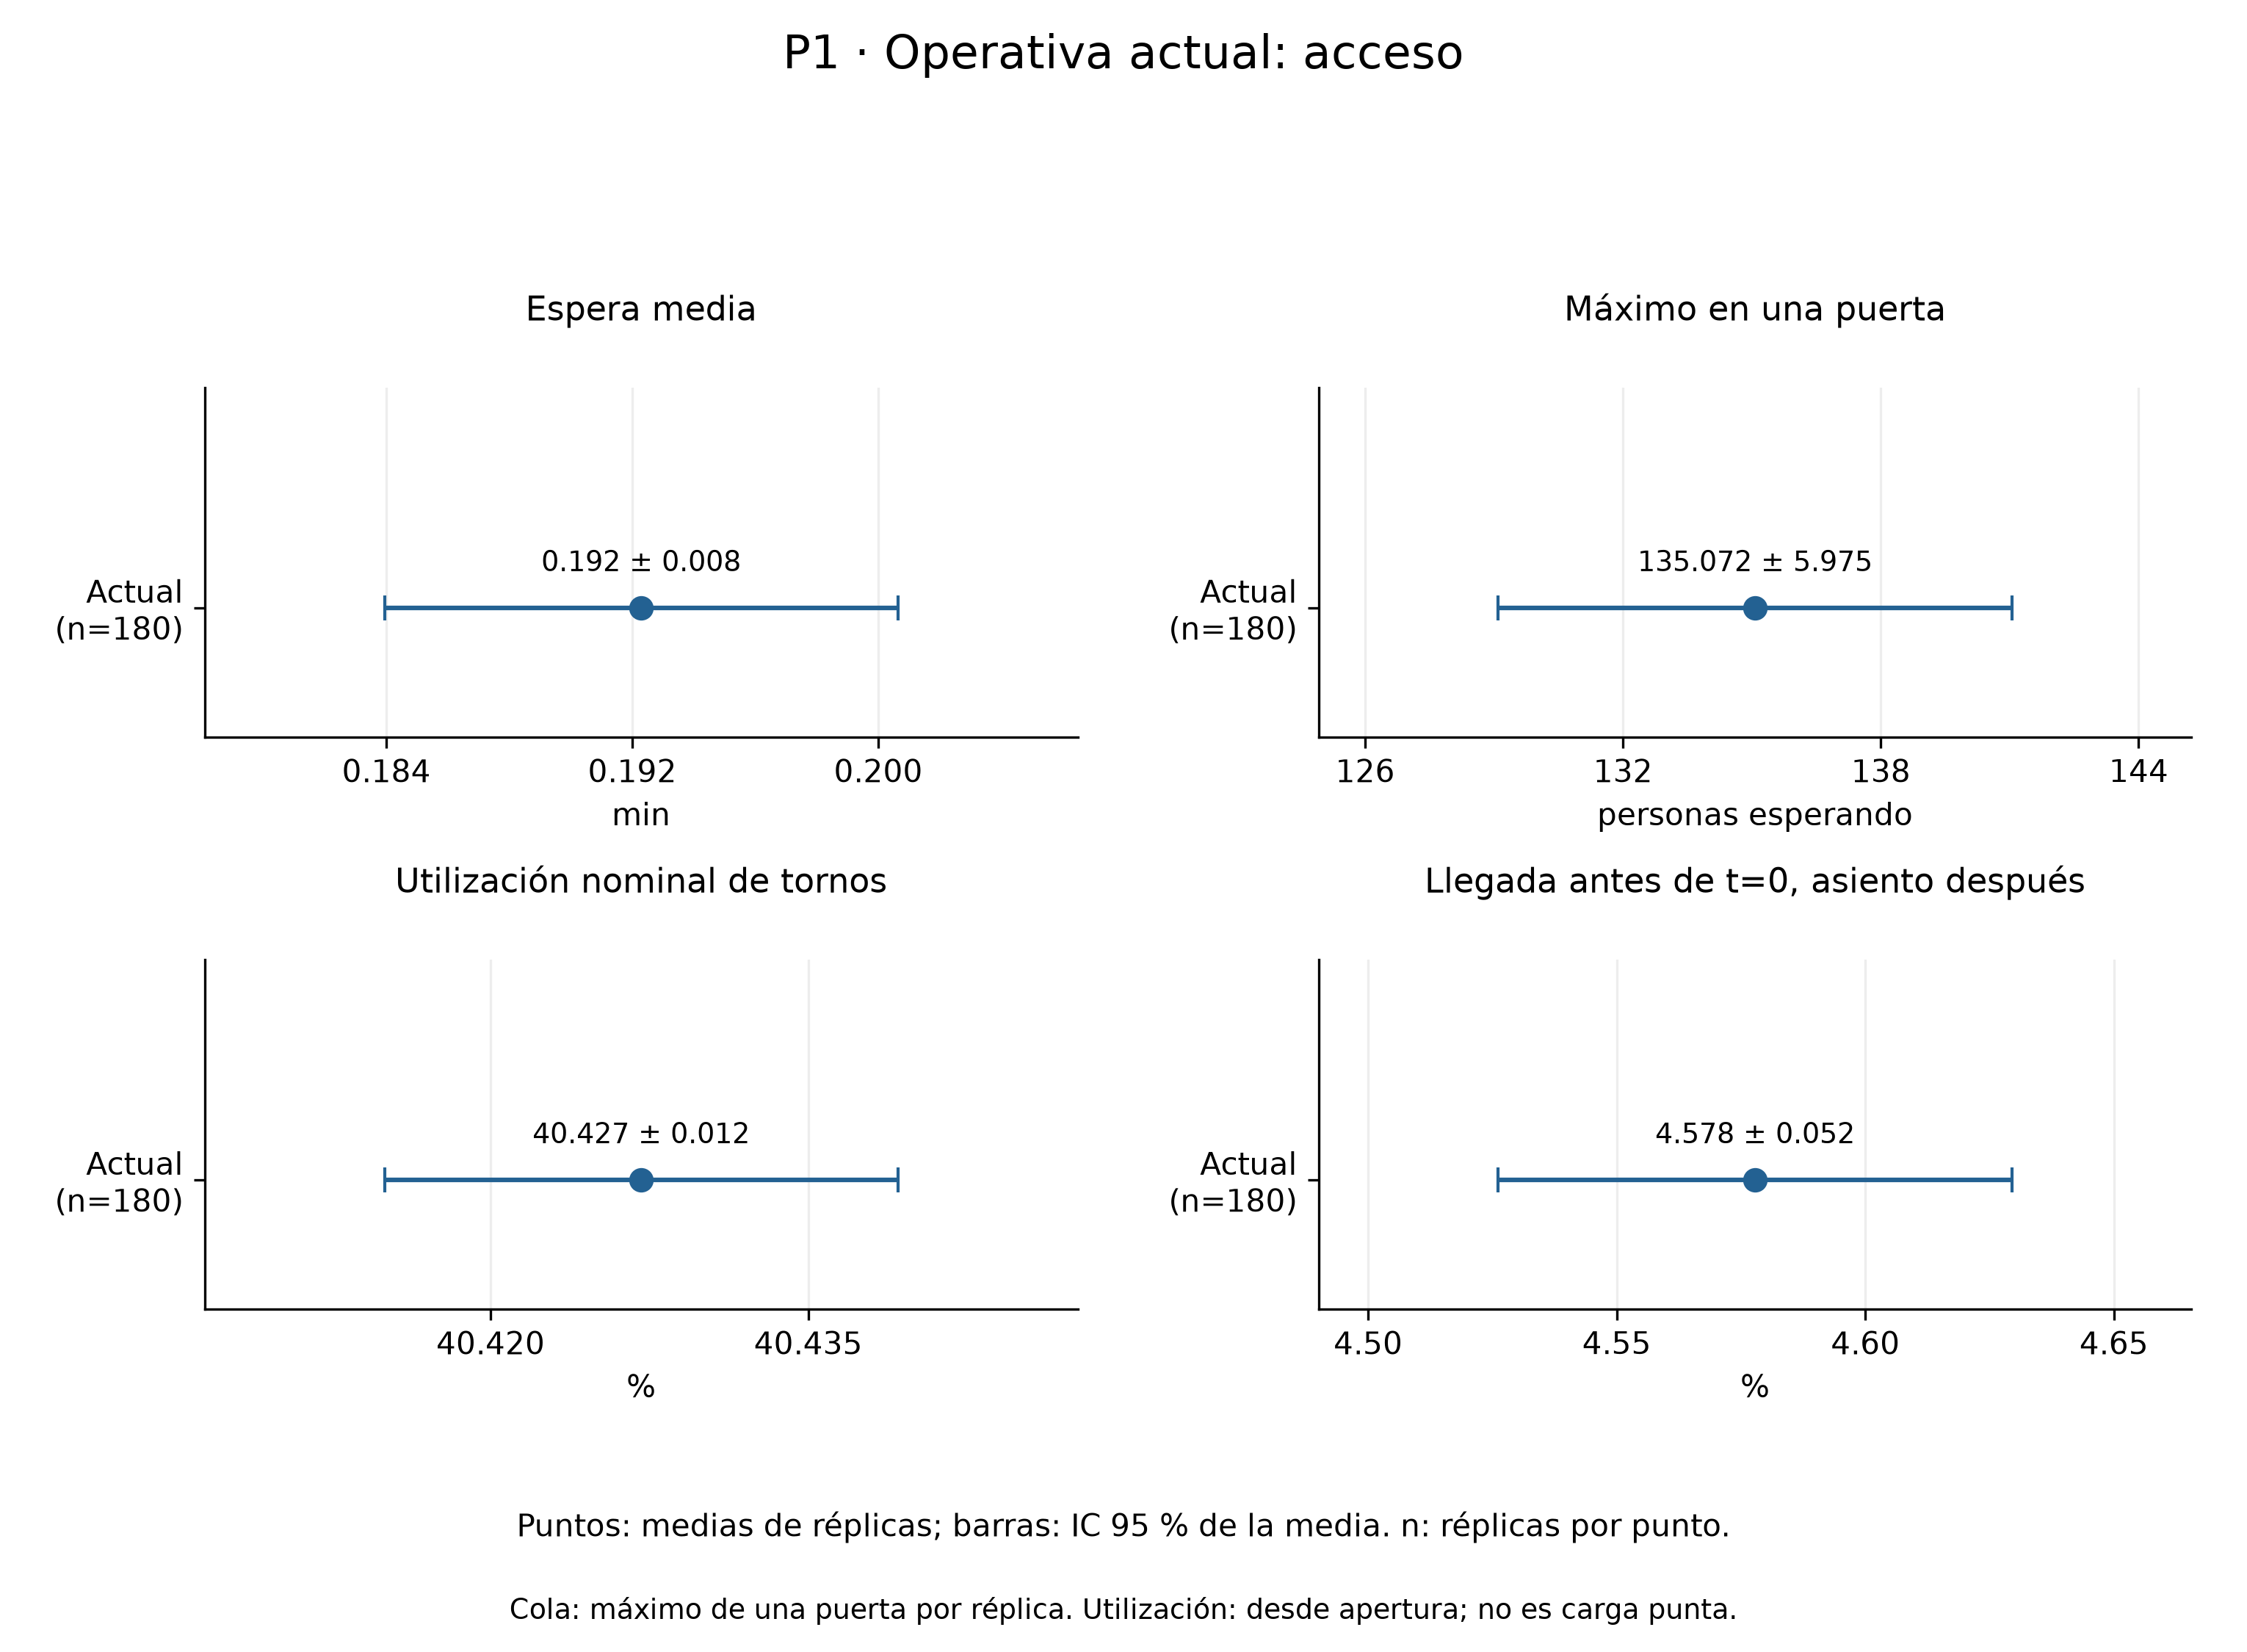
\includegraphics[width=\textwidth]{P1.png}
\caption{P1. Operativa actual (X0, $n=180$): espera media, máximo de personas
esperando en una puerta, utilización de los tornos y entrada tardía. Medias entre
réplicas con IC del 95~\%.}
\label{fig:p1}
\end{figure}

\textbf{Cuello de botella.} En la punta ($-30$ a 0~min) llegan 910~pers/min y los
72 tornos atienden 978: $\rho=0{,}93$. Los vomitorios admiten 411~pers/min por
macrozona frente a los 245 que dejan pasar los tornos, así que sin conflictos no
limitan la entrada. Con $\rho$ tan cerca de 1, pequeños cambios en la carga
tienen mucho efecto: con un 25~\% más de tiempo de servicio ($\rho=1{,}15$) la
espera media sube 1,217~$\pm$~0,034~min (30 parejas;
sección~\ref{sec:sensibilidad}).

\textbf{La entrada tardía no se debe sobre todo a la cola.} Con 4 tornos, donde la
espera es casi nula (0,016~$\pm$~0,001~min), sigue siendo del
3,754~$\pm$~0,016~\% ($n=183$); la diferencia emparejada con X0 es de
$-0{,}824 \pm 0{,}048$ puntos (180 parejas). Tampoco se debe a los conflictos: repitiendo X0 sin conflictos con las mismas
180 semillas, la entrada tardía baja del 4,578~\% al 4,488~\%, una diferencia
emparejada de 0,090~$\pm$~0,006 puntos, y el tiempo de acceso de 1,972 a
1,941~min, 0,032~$\pm$~0,001~min ($n=180$). Los conflictos explican menos del
2~\% de la entrada tardía. La mayor parte se explica, por tanto, por quienes
llegan en los últimos minutos y por el recorrido hasta el asiento.

\textbf{Resultado y supuestos.} Que los tornos sean el recurso más cargado y que la
espera sea corta con $\rho=0{,}93$ se sigue de los parámetros. Las cifras
absolutas dependen del número de tornos por puerta (3, una hipótesis de la Parte 1
porque el dato real no es público), del perfil de llegadas y del tiempo de
servicio, al que la espera es muy sensible.

\textbf{Limitaciones.} La utilización no describe la carga en la punta
(sección~\ref{sec:indicadores}) y los resultados agregados no permiten
reconstruir la cola a lo largo del reloj.

% ---------------------------------------------------------------------------
\subsection{P2 · Tornos por puerta}

\textbf{Respuesta.} Tres tornos por puerta, el valor actual, es el menor número
ensayado que cumple el objetivo de que el 95~\% del público espere menos de
10~minutos: con 3 y con 4 todo el público espera menos de 10~minutos en todas las
réplicas; con 2 no se alcanza el 95~\% en ninguna.

\begin{table}[htbp]
\centering\small
\caption{Tornos por puerta (X1 frente a X0).}
\label{tab:p2}
\begin{tabular}{@{}lrrrrrr@{}}
\toprule
Tornos & $n$ & $\rho$ & Espera $<$ 10~min & Espera media (min) & Percentil 95 (min) & Entrada tardía \\
\midrule
2 & 30 & 1,40 & 88,96 $\pm$ 0,74~\% & 4,016 $\pm$ 0,078 & 11,764 $\pm$ 0,266 & 20,30 $\pm$ 0,20~\% \\
3 & 180 & 0,93 & 100,0~\% & 0,192 $\pm$ 0,008 & 1,150 $\pm$ 0,068 & 4,58 $\pm$ 0,05~\% \\
4 & 183 & 0,70 & 100,0~\% & 0,016 $\pm$ 0,001 & 0,076 $\pm$ 0,002 & 3,75 $\pm$ 0,02~\% \\
\bottomrule
\end{tabular}
\end{table}

\begin{figure}[htbp]
\centering
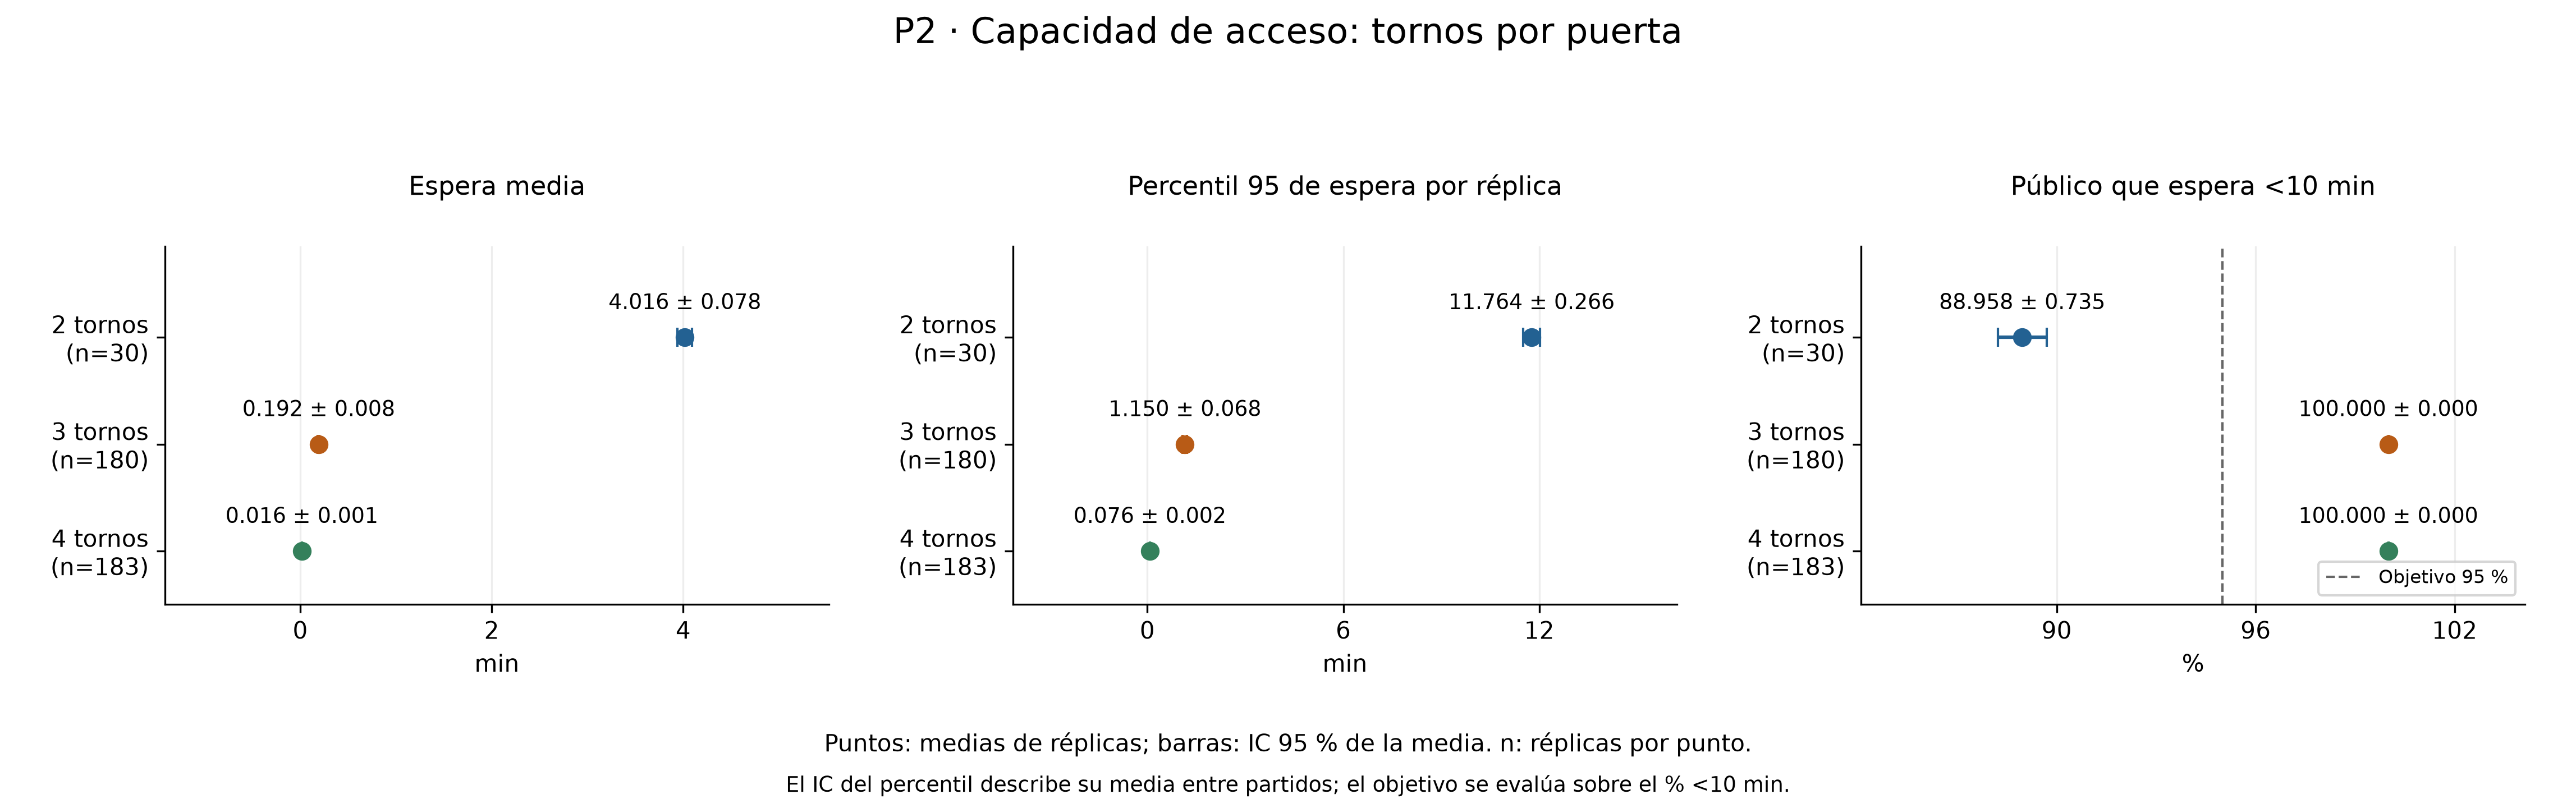
\includegraphics[width=\textwidth]{P2.png}
\caption{P2. Espera media, percentil 95 por réplica y público que espera menos
de 10~min con 2 ($n=30$), 3 ($n=180$) y 4 ($n=183$) tornos por puerta. Medias
con IC del 95~\%.}
\label{fig:p2}
\end{figure}

Con 2 tornos, el porcentaje que espera menos de 10~minutos va del 85,2~\% al
92,4~\% según la réplica: ninguna de las 30 llega al 95~\%. Frente a 3 tornos, la
espera media sube 3,832~$\pm$~0,067~min, el porcentaje bajo 10~minutos cae
11,04~$\pm$~0,74 puntos y la entrada tardía sube 15,79~$\pm$~0,19 puntos (30
parejas). La capacidad es menor que la demanda en la punta ($\rho=1{,}40$) y la
espera crece mientras dura, hasta unos 12~min; después la cola se vacía. Pasar de
3 a 4 tornos reduce la espera media en 0,176~$\pm$~0,008~min (unos 11~s) y la
entrada tardía en 0,82~$\pm$~0,05 puntos (180 parejas), pero no cambia el
cumplimiento del objetivo, que ya era del 100~\%.

\textbf{Robustez.} Con 3 tornos el objetivo se mantiene en las variantes de
sensibilidad: con un 10~\% más de público, 100,0~\% ($n=73$); con un 25~\% más
de tiempo de servicio ($\rho=1{,}15$), 99,931~$\pm$~0,045~\% ($n=30$), aunque el
percentil 95 sube a 4,919~$\pm$~0,211~min.

\textbf{Resultado y supuestos.} Que 2 tornos no basten y 3 sí es un resultado
robusto del modelo: se sigue de $\rho$ a un lado y otro de 1 y se mantiene en la
sensibilidad. El margen de 3 tornos depende del tiempo de servicio y del perfil
de llegadas, que son hipótesis.

\textbf{Limitaciones.} Solo se han ensayado 2, 3 y 4 tornos, iguales en todas las
puertas. El criterio se mide por partido simulado; que se cumpla en las 180
réplicas no garantiza que se cumpla en cualquier partido real.

% ---------------------------------------------------------------------------
\subsection{P3 · Llegada anticipada}

\textbf{Respuesta.} Si un 30~\% de quienes llegarían en los últimos 30~minutos
adelanta su llegada (X2), la espera media baja de unos 11,5 a unos 3~segundos y
la entrada tardía casi a la mitad, del 4,6~\% al 2,6~\%.

\begin{table}[htbp]
\centering\small
\caption{Llegada anticipada (X2, $n=138$) frente a X0 ($n=180$); diferencias con 138 parejas.}
\label{tab:p3}
\begin{tabular}{@{}lrrr@{}}
\toprule
Indicador & X0 & X2 & Diferencia X2 $-$ X0 \\
\midrule
Espera media (min) & 0,192 $\pm$ 0,008 & 0,050 $\pm$ 0,003 & $-$0,142 $\pm$ 0,009 \\
Percentil 95 de la espera (min) & 1,150 $\pm$ 0,068 & 0,209 $\pm$ 0,012 & $-$0,935 $\pm$ 0,078 \\
Máximo en la cola de una puerta & 135 $\pm$ 6 & 72 $\pm$ 5 & $-$63 $\pm$ 8 \\
Tiempo de acceso (min) & 1,972 $\pm$ 0,008 & 1,824 $\pm$ 0,003 & $-$0,149 $\pm$ 0,009 \\
Entrada tardía (\%) & 4,578 $\pm$ 0,052 & 2,604 $\pm$ 0,014 & $-$1,970 $\pm$ 0,054 p.\,p. \\
\bottomrule
\end{tabular}
\end{table}

\begin{figure}[htbp]
\centering
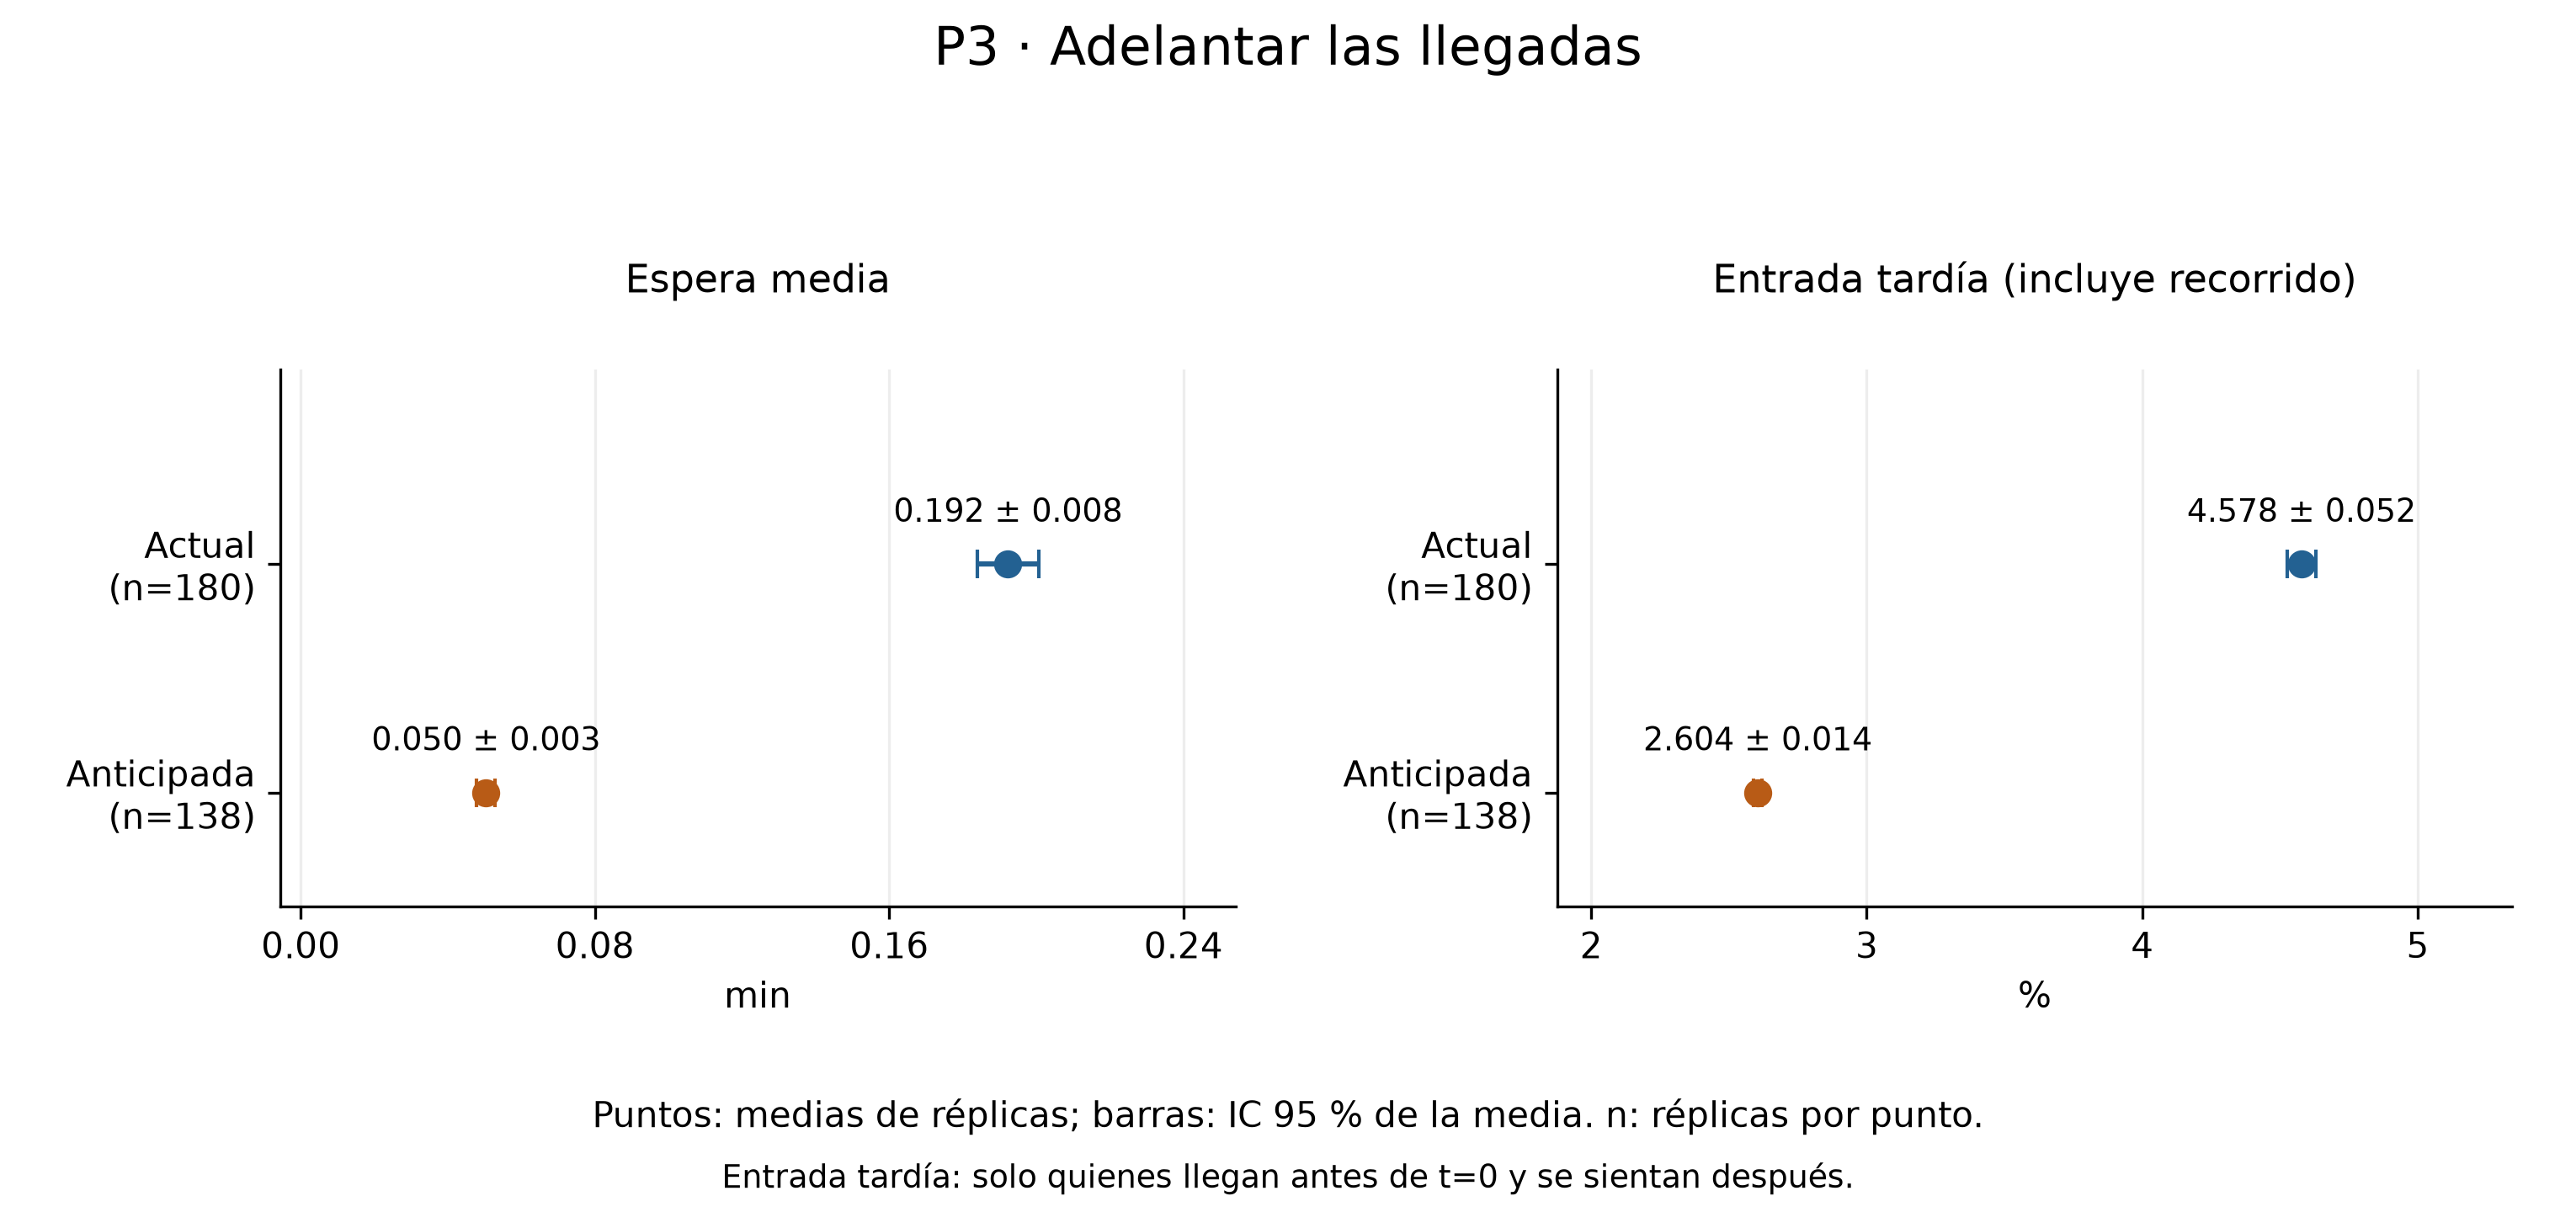
\includegraphics[width=0.92\textwidth]{P3.png}
\caption{P3. Espera media y entrada tardía con el perfil actual (X0, $n=180$) y
el anticipado (X2, $n=138$). Medias con IC del 95~\%. La entrada tardía incluye
el recorrido hasta el asiento.}
\label{fig:p3}
\end{figure}

La utilización no cambia (40,4~\%): el trabajo es el mismo, solo se reparte
mejor en el tiempo, y $\rho$ en la punta baja de 0,93 a 0,81. La entrada tardía
baja 1,97 puntos, más de lo que se gana al eliminar casi toda la cola con 4
tornos (0,82 puntos, P1): la mayor parte de la mejora viene de que menos gente
llega en los últimos minutos, no de la reducción de la cola. Esta lectura combina
dos contrastes distintos y es una inferencia, no una medida directa.

\textbf{Resultado y supuestos.} La dirección del efecto se sigue del modelo:
repartir las mismas llegadas en más tiempo reduce la carga en la punta. La
magnitud depende por completo del perfil anticipado, una hipótesis de la Parte 1
que no se ha calibrado con datos.

\textbf{Limitaciones.} El modelo no representa cómo se conseguiría que el público
llegue antes ni si un 30~\% es alcanzable. La mejora absoluta de la espera es
pequeña porque en X0 ya es corta; en un escenario más cargado, que no se ha
simulado, sería mayor.

% ---------------------------------------------------------------------------
\subsection{P4 · Prioridad para mayores y PMR}

\textbf{Respuesta.} Con prioridad no expulsiva en los tornos (X3), mayores y PMR
casi dejan de esperar (unos 11~s menos de media) y el resto espera unos 1,5~s
más; la espera media del conjunto no cambia.

\begin{table}[htbp]
\centering\small
\caption{Prioridad (mismos colectivos en X0, $n=180$, y X3, $n=181$; diferencias con 180 parejas).}
\label{tab:p4}
\begin{tabular}{@{}lrrr@{}}
\toprule
Colectivo & X0 (FIFO) & X3 (prioridad) & Diferencia X3 $-$ X0 \\
\midrule
Mayores y PMR, espera media (min) & 0,192 $\pm$ 0,008 & 0,0108 $\pm$ 0,0001 & $-$0,181 $\pm$ 0,008 \\
Resto, espera media (min) & 0,192 $\pm$ 0,008 & 0,217 $\pm$ 0,009 & $+$0,0248 $\pm$ 0,0011 \\
\bottomrule
\end{tabular}
\end{table}

\begin{figure}[htbp]
\centering
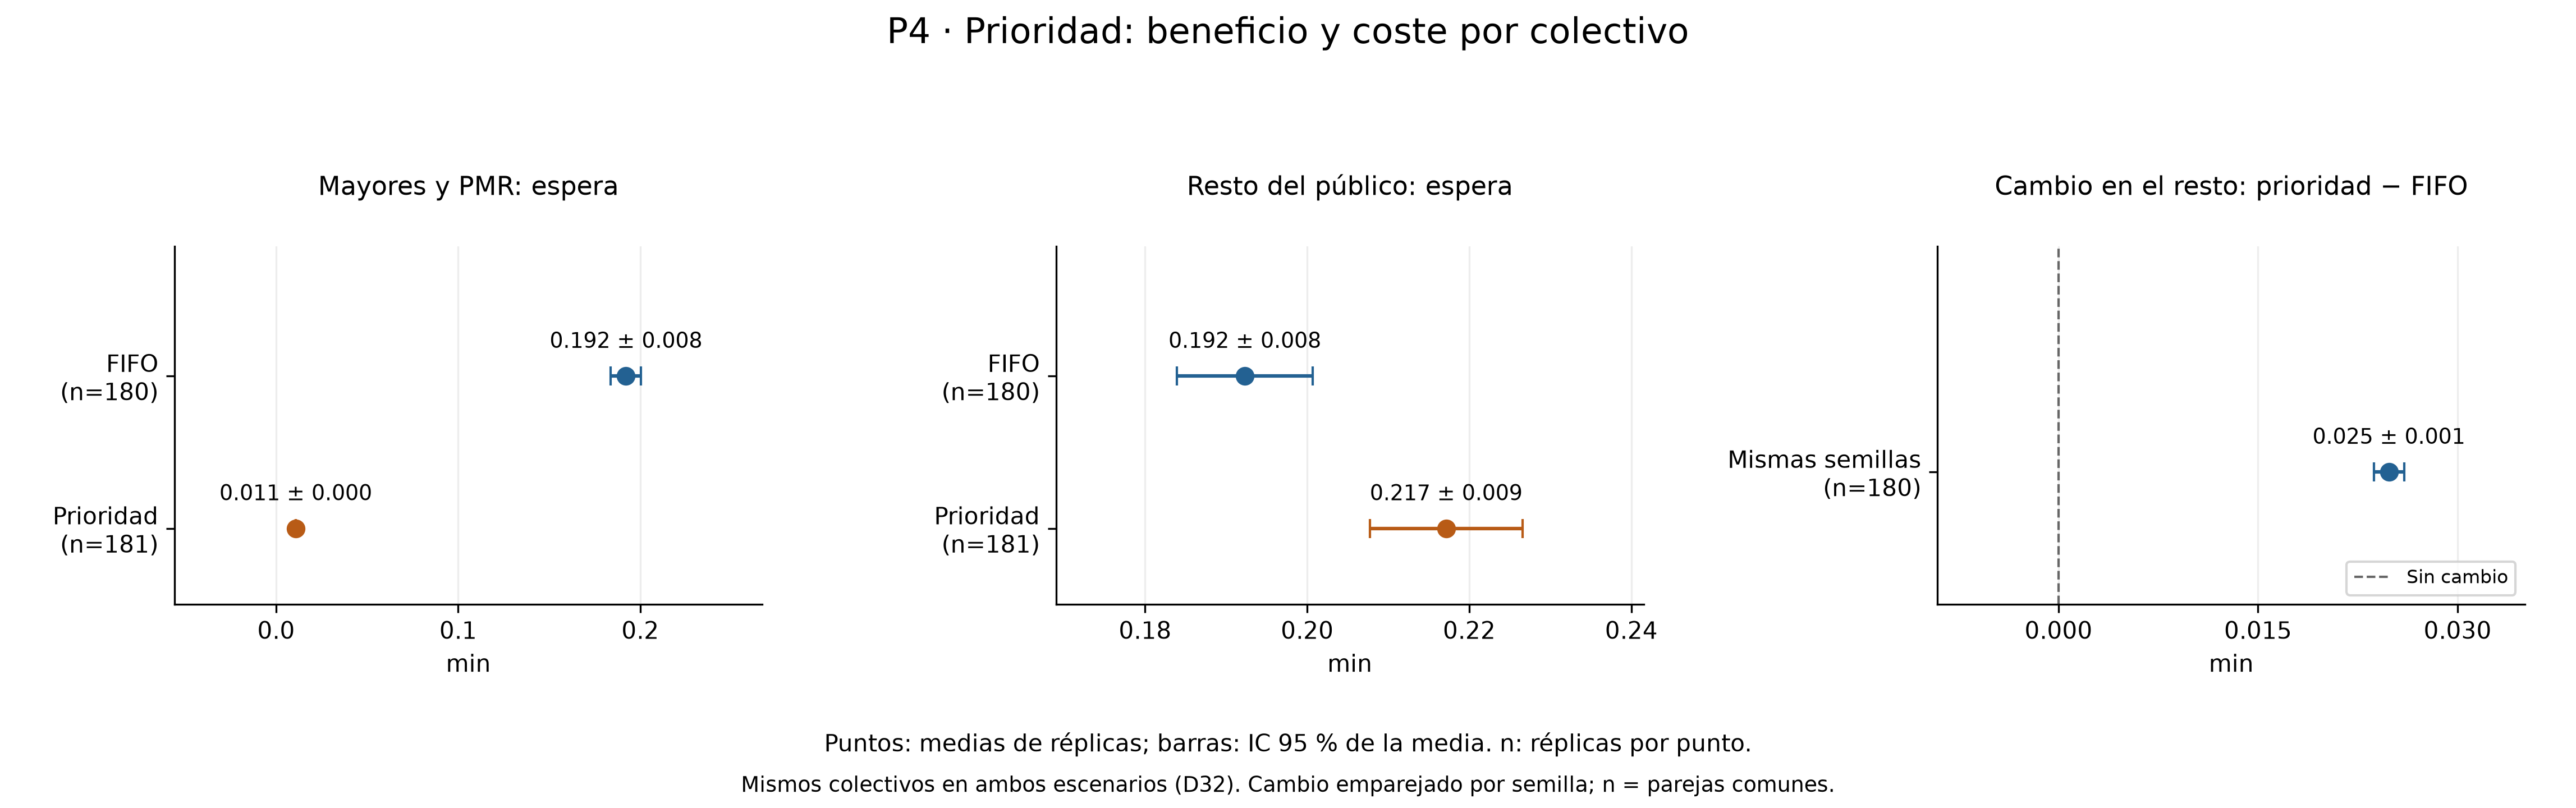
\includegraphics[width=\textwidth]{P4.png}
\caption{P4. Espera de mayores y PMR y del resto del público en FIFO (X0,
$n=180$) y con prioridad (X3, $n=181$), con los mismos colectivos; cambio
emparejado en el resto (180 parejas). Medias con IC del 95~\%.}
\label{fig:p4}
\end{figure}

En X3, la diferencia entre la espera de los priorizados y la del resto es de
$-0{,}206 \pm 0{,}009$~min ($n=181$). La espera media de todo el público no
cambia ($+0{,}00006 \pm 0{,}00007$~min; el intervalo incluye el cero), ni la
entrada tardía ($+0{,}0005 \pm 0{,}0028$ puntos): la prioridad reordena la cola
sin cambiar el trabajo de los tornos. La ganancia por persona priorizada es unas
siete veces la pérdida por persona del resto, porque el colectivo priorizado es
el 12~\% del público.

\textbf{Resultado y supuestos.} Que la espera total no cambie y que el coste se
reparta entre muchos es una propiedad de la prioridad no expulsiva con servicios
iguales. Las magnitudes absolutas son pequeñas porque la espera de X0 es corta;
con más carga, ganancia y pérdida serían mayores, pero no se ha simulado.

\textbf{Limitaciones.} La prioridad solo actúa en el torno, no en el vomitorio ni
en la salida. Se supone que el colectivo se identifica sin error ni coste al
llegar a la puerta. La movilidad reducida se representa solo con una velocidad
menor en el recorrido; el servicio en el torno es igual para todos.

% ---------------------------------------------------------------------------
\subsection{P5 · Salida escalonada}

\textbf{Respuesta.} Sí: con la salida escalonada (X4), el máximo de personas en
una salida baja casi a la mitad, a cambio de que el estadio tarde algo más de un
minuto más en vaciarse.

\begin{table}[htbp]
\centering\small
\caption{Salida simultánea (X0) frente a escalonada (X4), $n=180$ cada una; diferencias con 180 parejas.}
\label{tab:p5}
\begin{tabular}{@{}lrrr@{}}
\toprule
Indicador & Simultánea & Escalonada & Diferencia \\
\midrule
Máximo en una salida (personas) & 1.460,0 $\pm$ 1,3 & 746,1 $\pm$ 1,4 & $-$713,9 $\pm$ 0,6 \\
Vaciado desde el final del partido (min) & 8,367 $\pm$ 0,019 & 9,591 $\pm$ 0,108 & $+$1,224 $\pm$ 0,105 \\
\bottomrule
\end{tabular}
\end{table}

\begin{figure}[htbp]
\centering
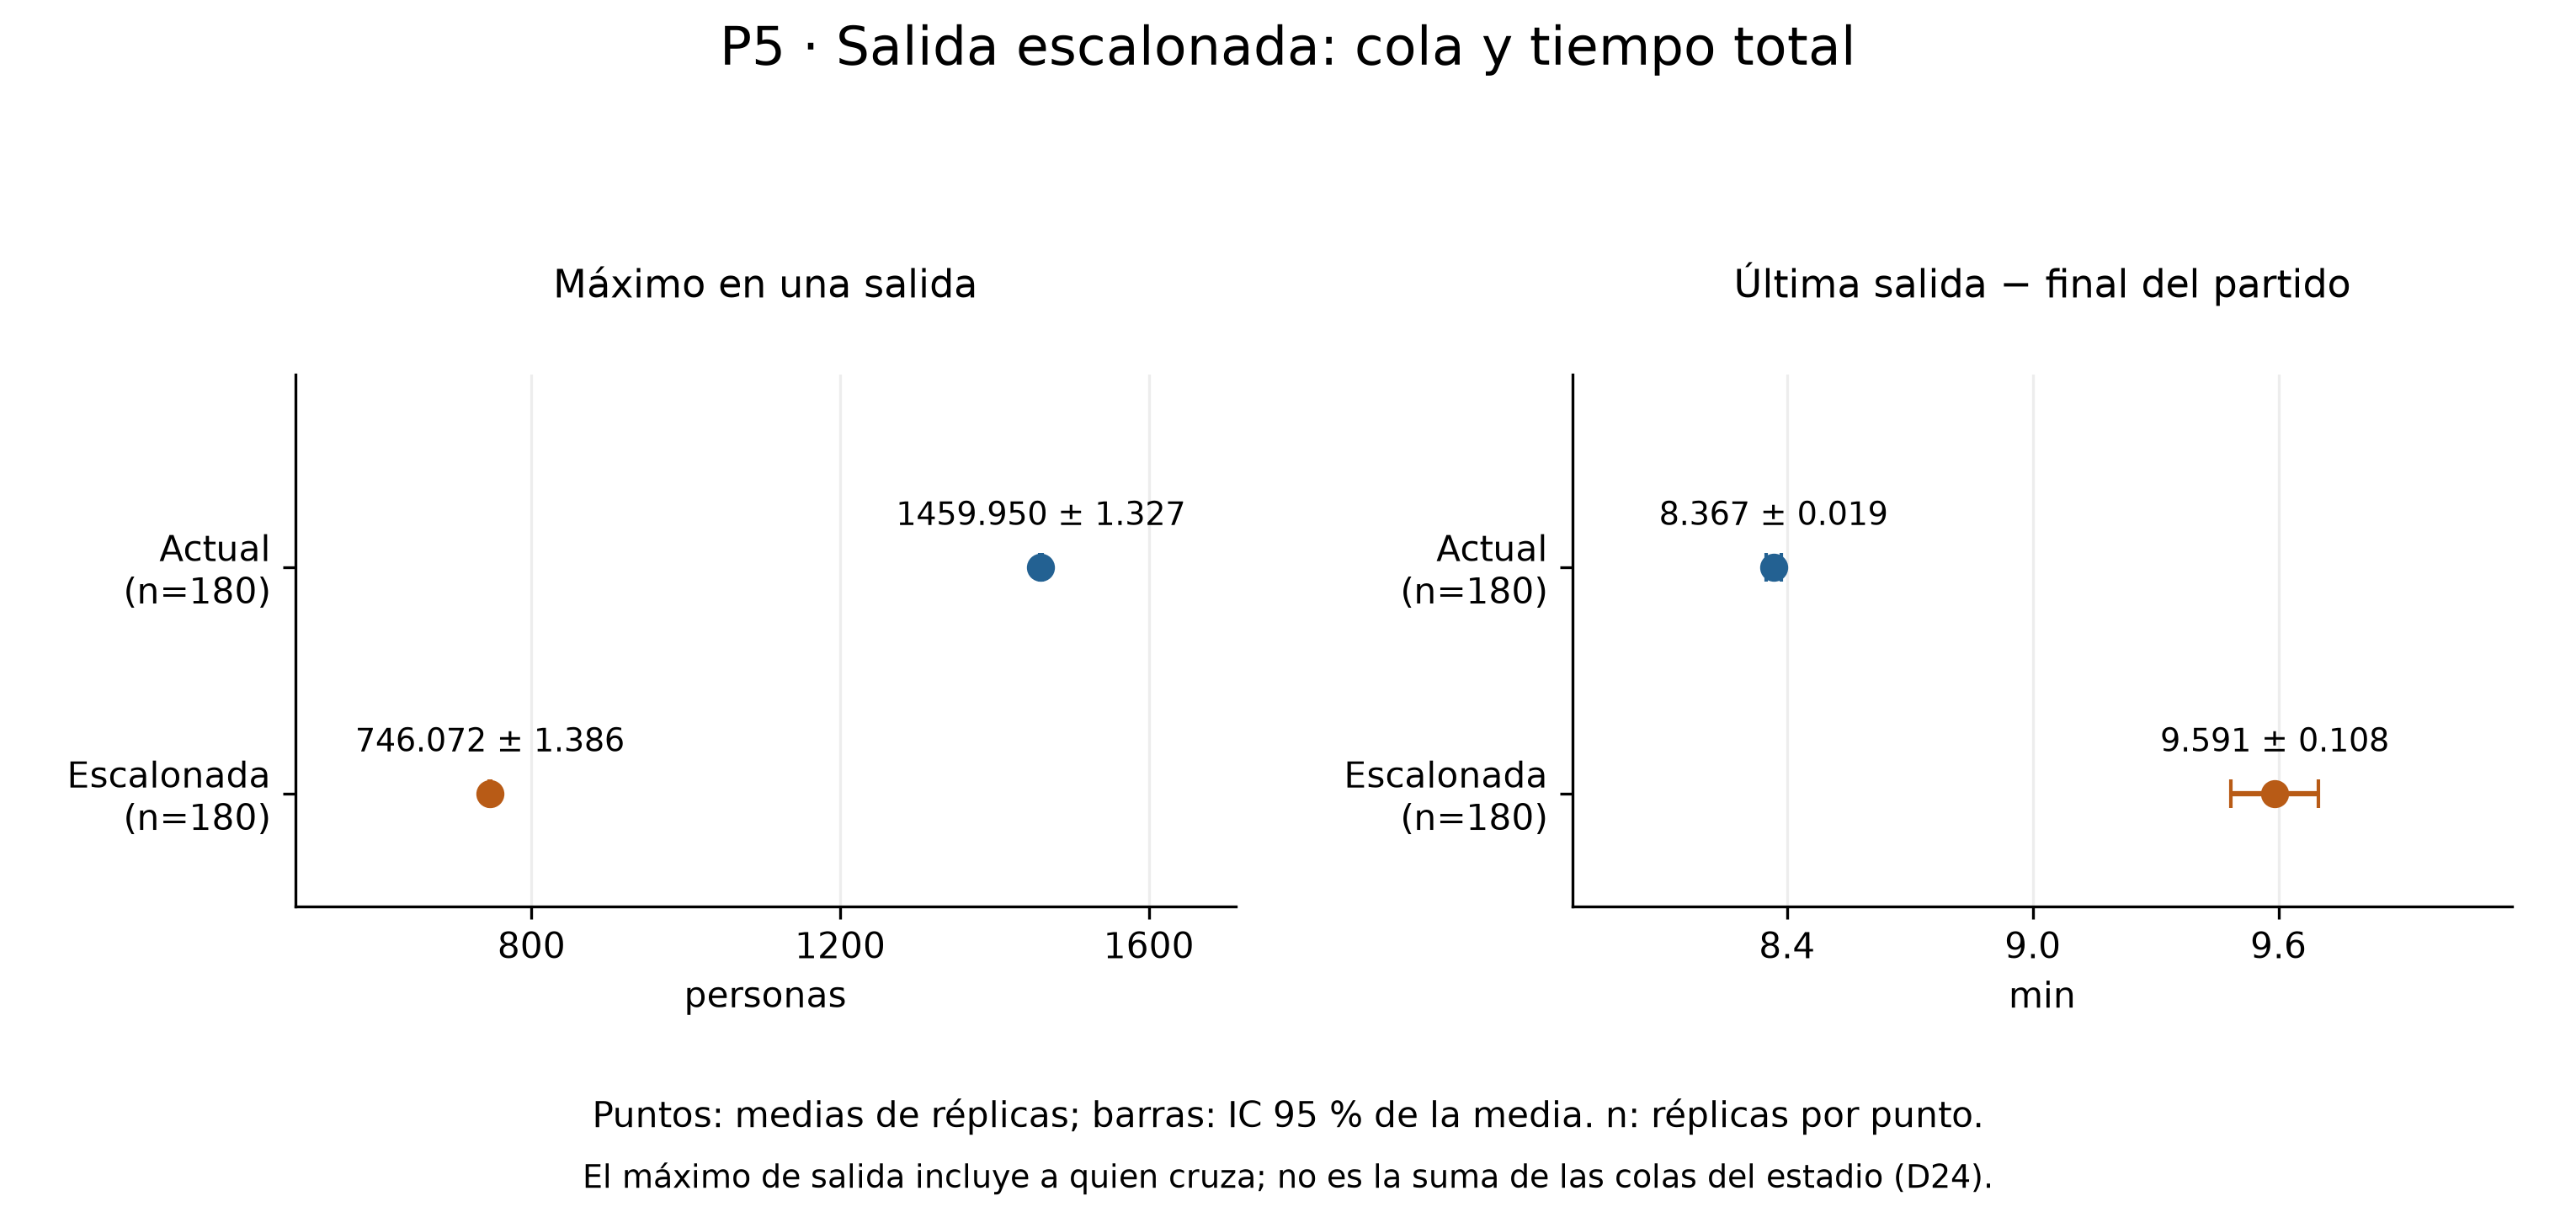
\includegraphics[width=0.92\textwidth]{P5.png}
\caption{P5. Máximo de personas en una salida y tiempo de vaciado con salida
simultánea (X0) y escalonada (X4), $n=180$ cada una. Medias con IC del 95~\%. El
máximo incluye a quien cruza la salida.}
\label{fig:p5}
\end{figure}

La salida escalonada reparte la carga en el tiempo: conviene si lo que preocupa
es la aglomeración en las salidas, no el tiempo total de vaciado. El máximo
incluye a quien está cruzando y no suma todas las colas del estadio. El vaciado
de X0 (8,367~min) supera los 7,7~min de la Parte 1 porque incluye la marcha hasta
la salida y la cola, que el cálculo de capacidad no considera.

% ---------------------------------------------------------------------------
\subsection{P6 · Conflictos por asiento y acomodadores}

\textbf{Respuesta.} Con conflictos al 1~\% el número de acomodadores es decisivo:
con 3 por macrozona el sistema se satura; con 6 todavía se forma cola, y de los
tres niveles probados solo con 9 la duración de un conflicto se acerca a la de la
propia resolución.

Con conflictos al 1~\% hay unos 490 conflictos por partido, unos 122 por
macrozona, concentrados en la hora punta, que exigen unos 569~min de trabajo de
acomodador por macrozona. Cada uno ocupa a un acomodador una media teórica de
4,67~min de resolución.

\begin{table}[htbp]
\centering\small
\caption{Acomodadores por macrozona con conflictos al 1~\% (X5, $n=180$ por nivel).}
\label{tab:p6}
\begin{tabular}{@{}lrrr@{}}
\toprule
Acomodadores & \makecell[r]{Duración media de\\un conflicto (min)} & \makecell[r]{Retraso al resto del\\bloque (s por persona)} & \makecell[r]{Entrada\\tardía (\%)} \\
\midrule
3 & 44,600 $\pm$ 0,477 & 291,7 $\pm$ 11,9 & 14,55 $\pm$ 0,28 \\
6 & 13,744 $\pm$ 0,206 & 36,8 $\pm$ 2,4 & 7,19 $\pm$ 0,14 \\
9 & 6,644 $\pm$ 0,092 & 6,7 $\pm$ 0,6 & 5,13 $\pm$ 0,07 \\
\bottomrule
\end{tabular}
\end{table}

\begin{figure}[htbp]
\centering
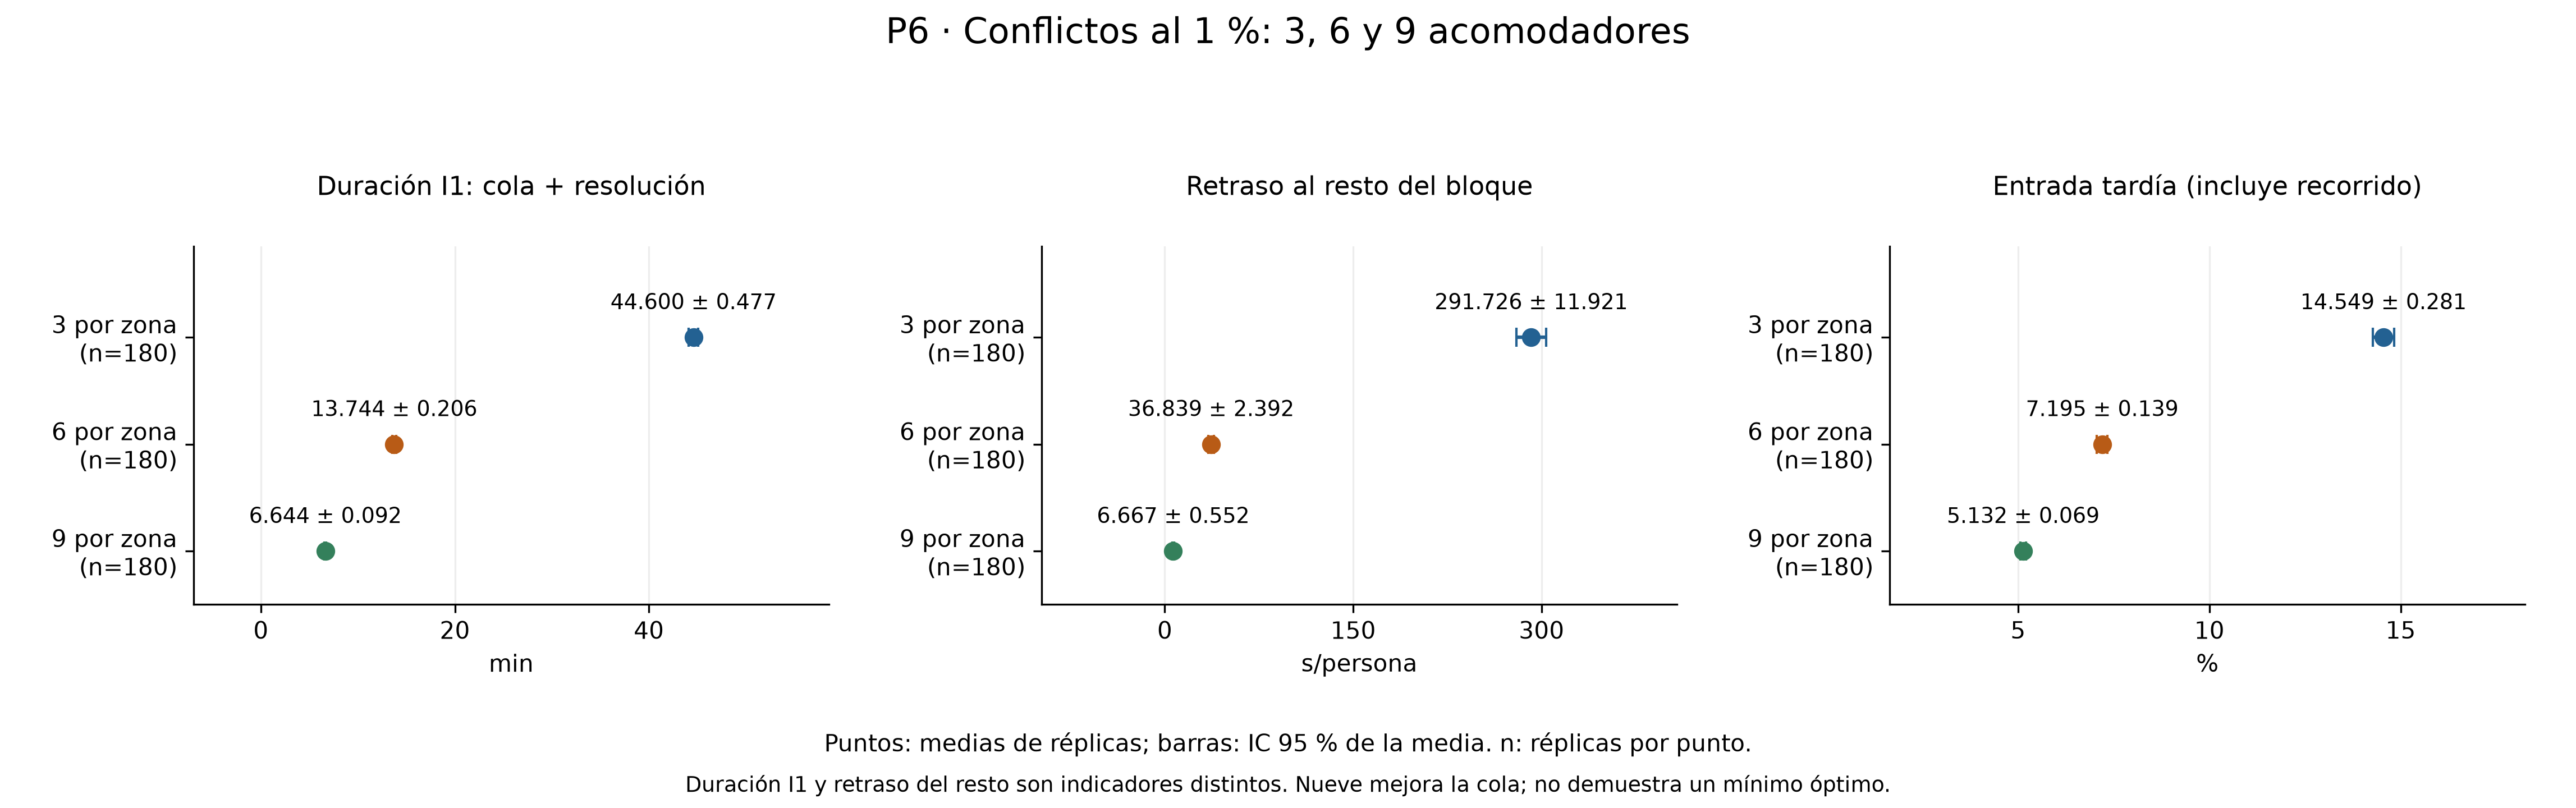
\includegraphics[width=\textwidth]{P6.png}
\caption{P6. Duración media de un conflicto (espera al acomodador más
resolución), retraso al resto del bloque y entrada tardía con 3, 6 y 9
acomodadores por macrozona ($n=180$ por nivel). Medias con IC del 95~\%.}
\label{fig:p6}
\end{figure}

Frente a 6 acomodadores, el retraso al resto del bloque aumenta
254,9~$\pm$~9,9~s por persona con 3 y baja 30,2~$\pm$~1,9 con 9 (180 parejas).
Con 3, los conflictos esperan mucho más de lo que tardan en resolverse y, en el
peor caso observado, el último espectador se sienta casi tres horas después del
inicio del partido. La duración media incluye la espera al acomodador, por eso
supera el rango de la resolución sin contradecir su distribución; con
acomodadores casi ilimitados vuelve a la media teórica (tabla~\ref{tab:limites}).

\textbf{Limitaciones.} El retraso al resto del bloque es una comparación entre
espectadores expuestos y no expuestos a un conflicto, no una medida causal del
mismo espectador con y sin conflicto. Nueve acomodadores mejoran mucho la
situación, pero no eliminan toda la cola ni demuestran que 9 sea el mínimo
necesario.

% ---------------------------------------------------------------------------
\subsection{P7 · Cierre de una puerta en hora punta}\label{sec:p7}

\textbf{Respuesta.} Sí, la redirección lo absorbe casi por completo. Si la puerta
A-1 se cierra 10~minutos al empezar la punta ($t=-30$), quienes llegan a ella
esperan de media unos 9,6~minutos sin redirección y medio minuto con ella.

El colectivo afectado son los asignados a A-1 que llegan durante el cierre:
383,3~$\pm$~5,6 de media sin redirección y 382,5~$\pm$~2,7 con ella; con
redirección se redirigen todos.

\begin{table}[htbp]
\centering\small
\caption{Cierre de A-1 en $[-30,-20)$~min: sin redirección ($n=45$) y con ella
($n=199$); diferencias con 45 parejas.}
\label{tab:p7}
\begin{tabular}{@{}lrrr@{}}
\toprule
Indicador & Sin redirección & Con redirección & Diferencia con $-$ sin \\
\midrule
Espera media del colectivo afectado (min) & 9,626 $\pm$ 0,120 & 0,543 $\pm$ 0,026 & --- \\
Espera media de todo el público (min) & 0,403 $\pm$ 0,018 & 0,243 $\pm$ 0,009 & $-$0,160 $\pm$ 0,007 \\
Máximo en la cola de una puerta & 395 $\pm$ 7 & 140 $\pm$ 6 & $-$258 $\pm$ 13 \\
Entrada tardía (\%) & 5,247 $\pm$ 0,108 & 4,645 $\pm$ 0,052 & $-$0,650 $\pm$ 0,029 p.\,p. \\
Público que espera $<$ 10~min (\%) & 99,717 $\pm$ 0,143 & 100,0 & $+$0,283 $\pm$ 0,143 \\
\bottomrule
\end{tabular}
\end{table}

\begin{figure}[htbp]
\centering
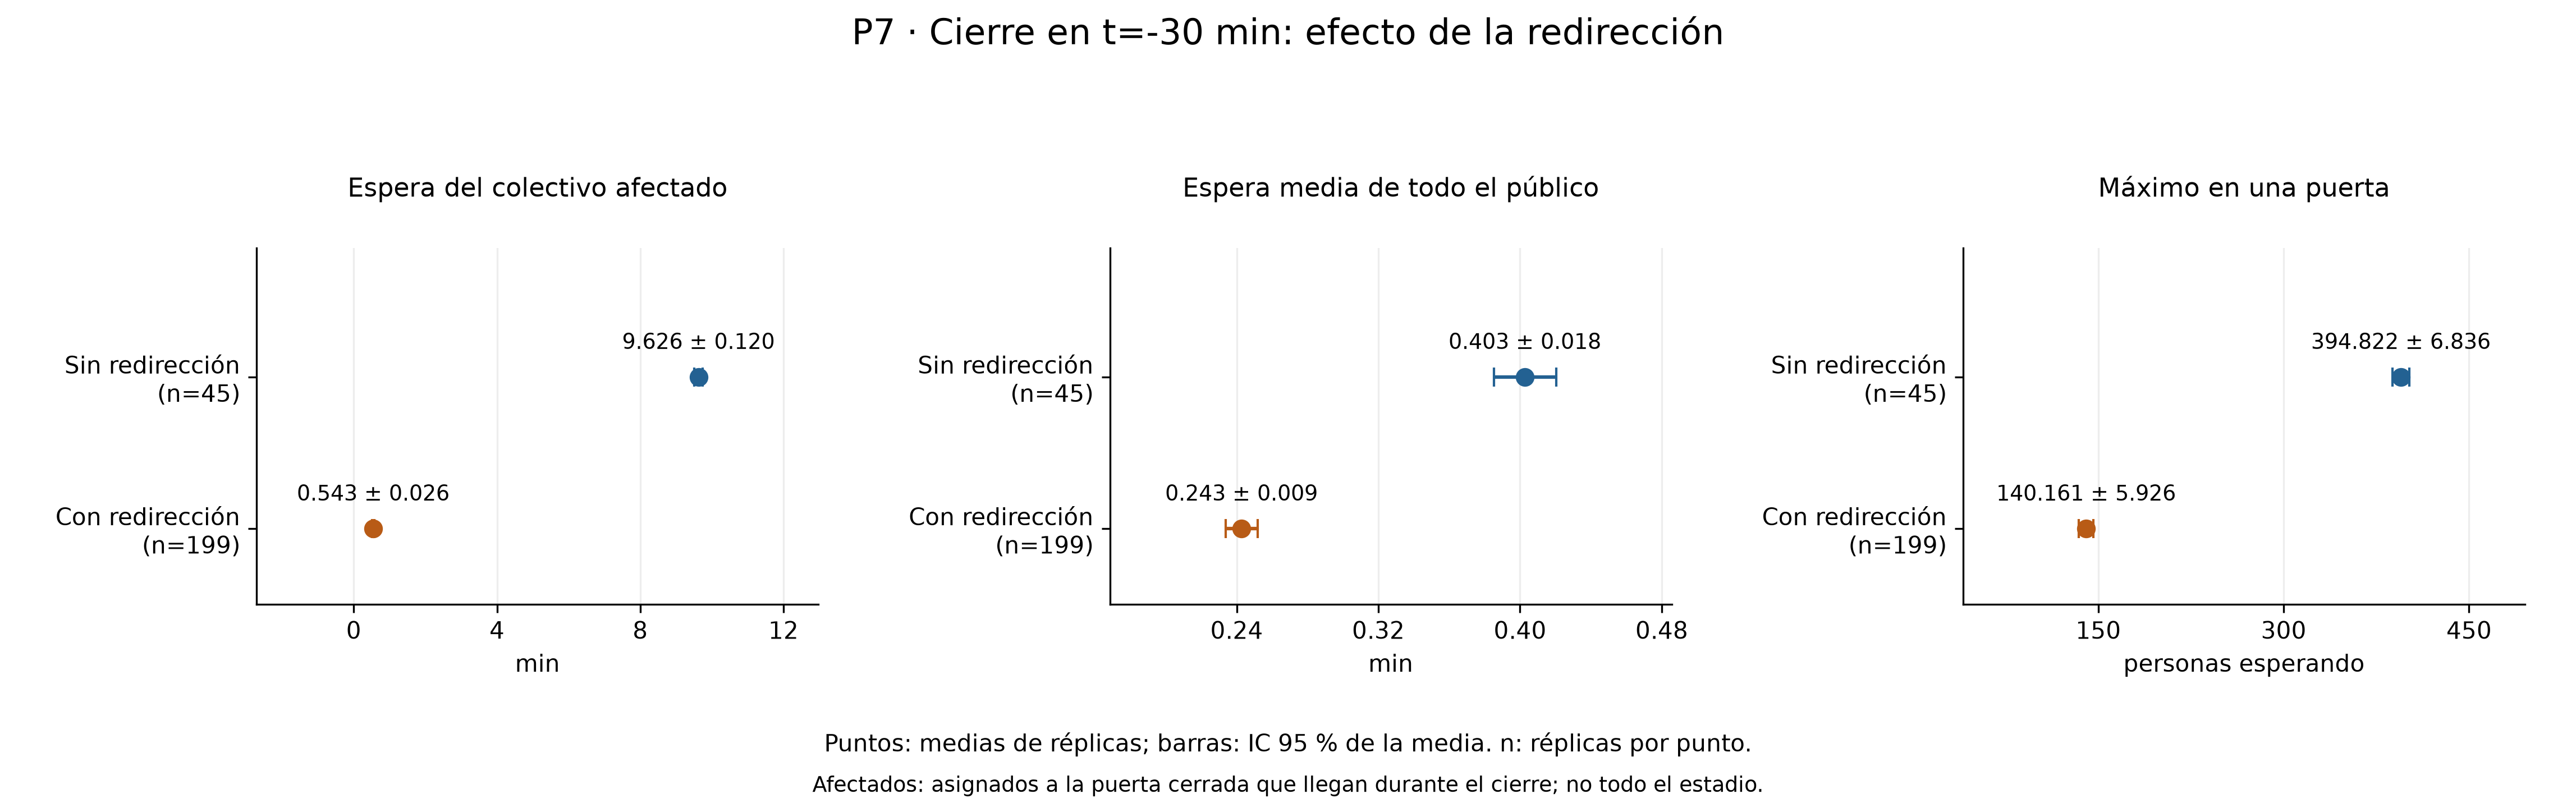
\includegraphics[width=\textwidth]{P7.png}
\caption{P7. Cierre de la puerta A-1 en $[-30,-20)$~min sin redirección ($n=45$) y
con ella ($n=199$): espera del colectivo afectado, espera media de todo el
público y máximo en una puerta. Medias con IC del 95~\%.}
\label{fig:p7}
\end{figure}

Sin redirección, quien llega al cerrar espera casi todo el cierre y quien llega
después se encuentra la cola acumulada; la espera observada coincide con la del
modelo fluido (apartado~\ref{sec:rho}). Con redirección, las otras cinco puertas
de la macrozona reciben un 20~\% más de llegadas durante 10~minutos, con holgura
suficiente ($\rho=0{,}93$), y la espera de los afectados se queda en medio
minuto. La redirección mitiga el cierre, pero no lo hace invisible: frente a X0
sin cierre, la espera media de todo el público con redirección es
$+0{,}050 \pm 0{,}003$~min mayor (180 parejas). El efecto se ve en el colectivo
afectado y en la cola máxima, no en las medias globales, porque el cierre afecta
a 1 de las 24 puertas.

\textbf{Resultado y supuestos.} Que la redirección absorba el cierre es un
resultado del modelo en estas condiciones: hay holgura en las demás puertas en
la punta. La magnitud depende de supuestos que la favorecen.

\textbf{Limitaciones.}
\begin{itemize}
  \item \textbf{Cola ya formada.} Según la hipótesis adoptada
    (sección~\ref{sec:desviaciones}), el cierre solo afecta a quien llega
    mientras dura. En $t=-30$ apenas hay cola formada, así que casi no influye;
    con cierres más tardíos la alternativa daría un efecto mayor, que no se ha
    medido.
  \item \textbf{Redirección optimista.} Quien llega a la puerta cerrada conoce al
    instante la cola de las demás, elige la menor y no camina ninguna distancia
    extra, porque el modelo no representa el exterior. Una redirección real
    costaría tiempo de desplazamiento y no sería perfecta.
  \item \textbf{Un solo caso.} Se ha estudiado una puerta, una duración (10~min) y
    un instante. En $t=+20$, el instante de la Parte 1, el cierre no tenía efecto
    apreciable.
  \item Sin redirección hay 45 réplicas frente a 199 con ella (tamaños por
    precisión); el contraste usa las 45 parejas comunes.
\end{itemize}

% ---------------------------------------------------------------------------
\subsection{P8 · Evacuación de emergencia}

\textbf{Respuesta.} Con todas las salidas el estadio se vacía de media en menos
de 8~minutos, pero no en todos los partidos: falla la marcha de una persona con
movilidad reducida, no la capacidad de las salidas. Con una salida bloqueada no
se cumple en ningún partido.

\begin{table}[htbp]
\centering\small
\caption{Evacuación con alarma en $t=+40$~min (X7, $n=180$ por variante).}
\label{tab:p8}
\begin{tabular}{@{}lrr@{}}
\toprule
Indicador & Todas las salidas & Una salida bloqueada \\
\midrule
Vaciado (min desde la alarma) & 7,469 $\pm$ 0,052 & 8,420 $\pm$ 0,014 \\
Personas a salvo a los 8~min (\%) & 99,9998 $\pm$ 0,0001 & 98,561 $\pm$ 0,028 \\
Partidos vaciados en $\le$ 8~min & 163 de 180 & 0 de 180 \\
\bottomrule
\end{tabular}
\end{table}

\begin{figure}[htbp]
\centering
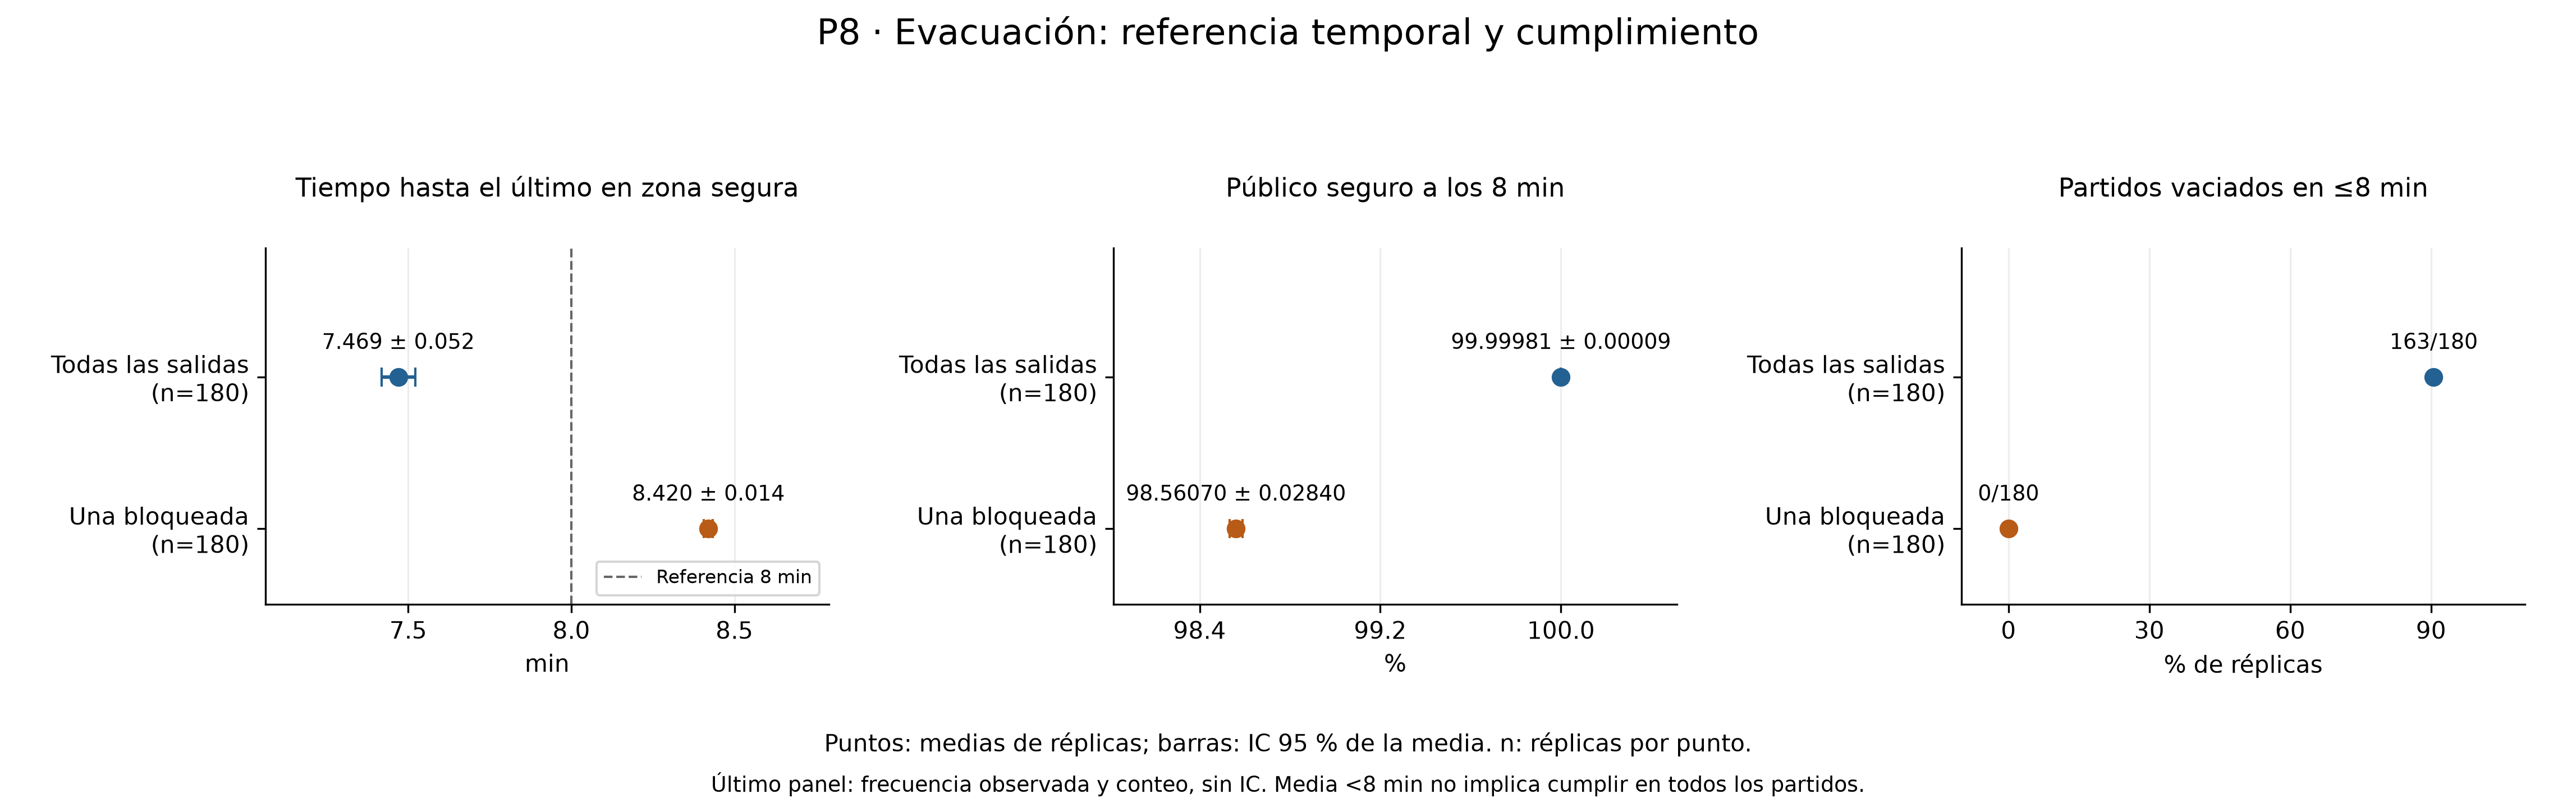
\includegraphics[width=\textwidth]{P8.png}
\caption{P8. Tiempo hasta que el último espectador está a salvo, porcentaje a
salvo a los 8~min y partidos vaciados en ese plazo, con todas las salidas y con
una bloqueada ($n=180$ por variante). Medias con IC del 95~\%; la frecuencia de
partidos se da como recuento, sin IC.}
\label{fig:p8}
\end{figure}

Una media inferior a 8~minutos no garantiza cumplir en cada partido. Con todas
las salidas, en las 17 réplicas que superan el plazo solo llega tarde una
persona, siempre PMR, lejos de la salida y sin hacer cola; sin las PMR, el
vaciado nunca pasa de 7,36~min. La capacidad de las salidas basta y el riesgo
está en evacuar a tiempo a las personas con movilidad reducida. Con una salida
bloqueada sí falla la capacidad: las 5 salidas restantes de la macrozona A no dan
abasto, aunque a los 8~minutos ya está a salvo el 98,56~\% de quienes evacúan.

Estos tiempos son mayores que los 5,9 y 7,1~min de la Parte 1 porque incluyen la
reacción y la marcha hasta la salida, que el cálculo de capacidad excluye.

\textbf{Limitaciones.} No se ha simulado ningún dispositivo de asistencia a las
PMR, así que su eficacia no se puede dar por demostrada. La alarma suena en un
único instante ($t=+40$), con todo el público dentro, y el modelo no representa
densidades, empujones ni bloqueos entre peatones.
